\documentclass[]{scrreprt}
\usepackage{amsmath,amsfonts,graphicx}

\def\species{\mathrm{sp}}
\def\phase{\mathrm{ph}}
\def\massfrac{\chi}
\def\flux{\mathbf{F}}
\def\darcyvel{\mathbf{v}}
\def\energydens{\mathcal{E}}
\def\d{\mathrm{d}}

\newcommand{\uo}{\mbox{UO\textsubscript{2}}\xspace}

\setcounter{secnumdepth}{3}


\begin{document}


\title{Newton-Cooling Tests}
\author{CSIRO}
\maketitle

\tableofcontents

\chapter{Classic Newton cooling in a bar}

Without fluids, mechanical deformation and sinks, the heat equation is
\begin{equation}
\rho_{R}C_{R}(1-\phi)\dot{T} = \nabla\lambda\nabla T \ ,
\end{equation}
where $\phi$ is the porosity, $\rho_{R}$ is the rock grain density
(kg.m$^{-3}$), $C_{R}$ is the rock grain specific heat capacity
(J.kg$^{-1}$.K$^{-1}$), $T$ is the temperature, and $\lambda$ is the
tensorial thermal conductivity of the porous material
(J.s$^{-1}$.K$^{-1}$.m$^{-1}$).

In section~\ref{pp.sec}, the dynamics of this equation is explored,
while this section concentrates on the steady-state situation.
Consider the one-dimensional case where a bar sits between $x=0$ and
$x=L$ with a fixed temperature at $x=0$:
\begin{equation}
T(x=0, t) = T_{0} \ ,
\end{equation}
and a sink flux at the other end:
\begin{equation}
\mbox{sink strength (J.m$^{-2}$.s$^{-1}$)} = \left.\lambda\frac{\partial
  T}{\partial x}\right|_{x=L} = -C\left(T - T_{e}\right)_{x=L} \ .
\label{eqn.heat.sink}
\end{equation}
Here $T_{e}$ is a fixed quantity (``e'' stands for ``external''), and
$C$ is a constant conductance (J.m$^{-2}$.s$^{-1}$.K$^{-1}$).

The solution is the linear function
\begin{equation}
T = T_{0} + \frac{T_{e} - T_{0}}{\lambda + C L} C x \ .
\end{equation}
The heat sink in Eqn~(\ref{eqn.heat.sink}) is a linear function of
$T$, so the {\tt PorousFlowPiecewiseLinearSink} may be employed.

The simulation is run in MOOSE using $C=1$, $L=100$, $\lambda=100$,
$T_{0}=2$ and $T_{e}=1$.  The solution is shown in Figure~\ref{nc_heat.fig}

\begin{figure}[htb]
\begin{center}
\includegraphics[width=16cm]{nc_temp.pdf}
\caption{The steady-state temperature in the bar.  MOOSE agrees well
  with theory illustrating that piecewise-linear heat sinks/sources
  and heat conduction are correctly implemented in MOOSE.}
\label{nc_heat.fig}
\end{center}
\end{figure}


\chapter{Porepressure sink in a bar}
\label{pp.sec}

These tests demonstrate that MOOSE behaves correctly when a simulation
contains a sink.  The sink is a piecewise linear function of pressure.

Darcy's equation for (single-phase) flow through a fully saturated medium without
gravity and without sources is
\begin{equation}
\frac{\partial}{\partial t}\phi\rho = \nabla_{i}\left(\frac{\rho
  \kappa_{ij}}{\mu} \nabla_{j}P \right) \ ,
\end{equation}
with the following notation:
\begin{itemize}
\item $\phi$ is the medium's porosity;
\item $\rho$ is the fluid density;
\item $\kappa_{ij}$ is the permeability tensor;
\item $\mu$ is the fluid viscosity;
\item $\partial/\partial t$ and $\nabla_{i}$ denote the time and spatial derivatives, respectively.
\end{itemize}
Using $\rho \propto
\exp(P/B)$, where $B$ is the fluid bulk modulus, Darcy's equation
becomes
\begin{equation}
\frac{\partial}{\partial t}\rho = \nabla_{i}\alpha_{ij}\nabla_{j}\rho \ ,
\end{equation}
with
\begin{equation}
\alpha_{ij} = \frac{\kappa_{ij}B}{\mu\phi} \ .
\end{equation}
Here the porosity and bulk modulus are assumed to be constant in space
and time.

Consider the one-dimensional case where a bar sits between $x=0$ and
$x=L$ with initial pressure distribution so $\rho(x,t=0) = \rho_{0}(x)$.
Maintain the end $x=0$ at constant pressure, so that $\rho(x=0, t) =
\rho_{0}(0)$.  At the end $x=L$, prescribe a sink flux
\begin{equation}
\left.\frac{\partial\rho}{\partial x}\right|_{x=L} = -C\left(\rho -
\rho_{e}\right)_{x=L} \ ,
\end{equation}
where $\rho_{e}$ is a fixed quantity (``e'' stands for ``external''),
and $C$ is a constant conductance.  This corresponds to the flux
\begin{equation}
\left.\frac{\partial P}{\partial x}\right|_{x=L} = -CB\left(1 -
e^{(P_{e}-P)/B}\right)_{x=L} \ ,
\end{equation}
which can easily be coded into a MOOSE input file: the flux is
$\rho\kappa\nabla P/\mu = -CB\kappa(e^{P/B} - e^{P_{e}/B})/\mu$, and
this may be represented by a piecewise linear function of pressure.

The solution of this problem is well known and is
\begin{equation}
\rho(x, t) = \rho_{0}(0) - \frac{\rho_{0}(0) - \rho_{e}}{1 + LC}Cx +
\sum_{n=1}^{\infty} a_{n}\sin \frac{k_{n}x}{L}e^{-k_{n}^{2}\alpha
  t/L^{2}} \ ,
\end{equation}
where $k_{n}$ is the $n^{\mathrm{th}}$ positive root of the equation
$LC\tan k + k=0$  ($k_{n}$ is a little bigger than
$(2n-1)\pi/2$), and $a_{n}$ is determined from
\begin{equation}
a_{n}\int_{0}^{L}\sin^{2}\frac{k_{n}x}{L}\,\mathrm{d}x =
\int_{0}^{L}\left(\rho_{0}(x) - \rho_{0}(0) + \frac{\rho_{0}(0) -
  \rho_{e}}{1 + LC}Cx\right)\sin \frac{k_{n}x}{L}\,\mathrm{d}x \ ,
\end{equation}
which may be solved numerically (Mathematica is used to generate
the solution in Figure~\ref{nc.fig}).

\noindent The problem is solved in MOOSE using the following parameters:
\begin{center}
\begin{tabular}{|ll|}
\hline
Bar length & 100\,m \\
Bar porosity & 0.1 \\
Bar permeability & $10^{-15}$\,m$^{2}$ \\
\hline
Gravity & 0 \\
\hline
Water density & 1000\,kg.m$^{-3}$ \\
Water viscosity & 0.001\,Pa.s \\
Water bulk modulus & 1\,MPa \\
\hline
Initial porepressure $P_{0}$ & 2\,MPa \\
Environmental pressure $P_{e}$ & 0 \\
\hline
Conductance $C$ & 0.05389\,m$^{-1}$ \\
\hline
\end{tabular} \\
\end{center}
This conductance is chosen so at steadystate $\rho(x=L)=2000$\,kg.m$^{-3}$.

The problem is solved using 1000 elements along the $x$ direction
($L=100$\,m), and using 100 time-steps of size $10^6$\,s.  Using fewer
elements or fewer timesteps means the agreement with the theory is
marginally poorer.  Two tests are performed: one with transient flow,
and one using the steadystate solver.  In this case the initial
condition is $P=2-x/L$\,MPa, since the uniform $P=2$\,MPa does not
converge.  The results are shown in Figure~\ref{nc.fig}.

\begin{figure}[htb]
\begin{center}
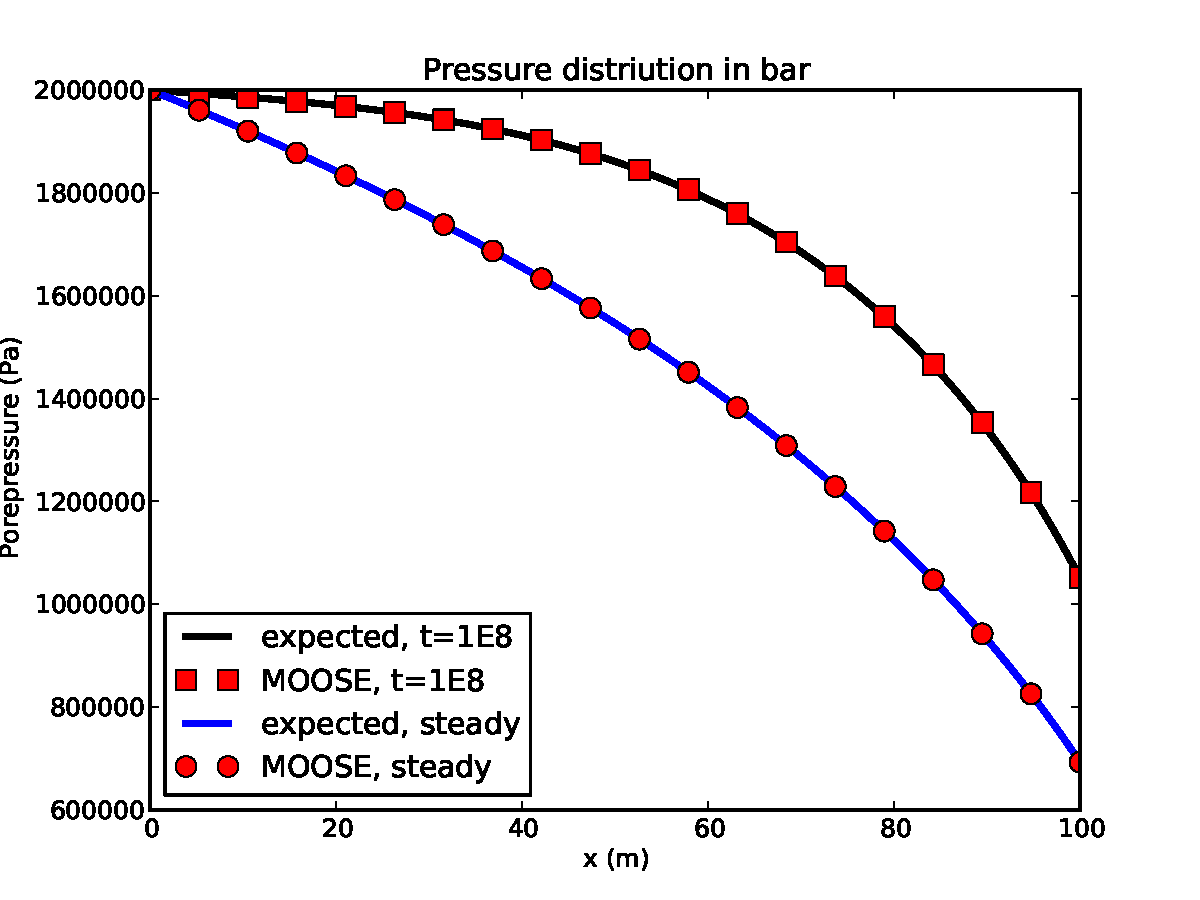
\includegraphics[width=17cm]{nc.pdf}
\caption{The porepressure in the bar at $t=10^{8}$\,s, and at
  steadystate.  The pressure at $x=0$ is held fixed, while the sink is
  applied at $x=100$\,m.  MOOSE agrees well with theory demonstrating
  that piecewise-linear sinks/sources and single-phase Darcy fluid
  flow are correctly implemented in MOOSE.}
\label{nc.fig}
\end{center}
\end{figure}


\chapter{Porepressure sink in a bar with heat}
\label{pp.heat.sec}

The simulation of Section~\ref{pp.sec} is re-run, but this time
heat flow is included.  In this section it is assumed that the fluid
specific enthalpy (J.kg$^{-1}$) is exactly equal to the fluid internal
energy, and that internal energy is ideal:
\begin{equation}
h = {\mathcal E} = C_{v}T \ .
\end{equation}
This makes the arguments below simple without having to consider real
fluids with complicated enthalpy and density expressions.

At the left end of the bar, the temperature is kept fixed:
\begin{equation}
T(x=0, t) = T_{0} \ .
\end{equation}
At the other end of the bar, heat is removed only by the fluid flowing
out of the system.  That is, there is a heat sink:
\begin{equation}
\mbox{sink strength (J.m$^{-2}$.s$^{-1}$)} = -C {\mathcal E}\left(\rho -
\rho_{e}\right)_{x=L} \ .
\end{equation}
No other sinks or sources are applied to the heat equation.

With this setup, the steady-state temperature in the bar must be
exactly
\begin{equation}
T(x, t=\infty) = T_{0} \ .
\end{equation}
For consider the fluid flowing from $x=0$ to $x=L$ in order to assume
steady-state.  At $x=0$ it must have temperature $T_{0}$ because that
temperature is fixed at $x=0$.  It advects this temperature with it as
it moves, so therefore at $t=\infty$, this temperature has permeated
throughout the entire bar.  This occurs even without heat conduction,
and is independent of the initial temperature of the bar.

MOOSE produces this result exactly.


\chapter{Hot ideal fluid in a bar}

This test uses a similar setup to Section~\ref{pp.heat.sec}, except
that here an ideal fluid is used.  The use of an ideal gas simplifies
the equations.  Only the steady-state is studied in this section.

The governing equation for the fluid's porepressure $P$ is
\begin{equation}
\nabla \frac{\rho\kappa}{\mu}\nabla P = 0 \ .
\end{equation}
It is assumed that $\kappa$ and $\mu$ are constant, and that
\begin{equation}
\rho = \frac{MP}{RT} \ ,
\end{equation}
holds (this is the ideal gas equation of state).  In this formula $M$
is the gas molar mass, $R$ is the gas constant and $T$ is the
temperature.

The equation governing the temperature is assumed to be just the fluid
advection equation
\begin{equation}
\nabla\frac{h\rho\kappa}{\mu}\nabla P = 0 \ .
\end{equation}
As in Section~\ref{pp.heat.sec}, heat conduction could be added, but
it is actually irrelevant since the solution to the problem below is
constant $T$.  The enthalpy, $h$, for an ideal gas is
\begin{equation}
h = C_{v}T + \frac{P}{\rho} = C_{v}T + \frac{RT}{M} = C_{p}T \ .
\end{equation}

The boundary conditions at the left-hand end are
\begin{equation}
P(x=0) = P_{0} \ \ \ \mbox{and}\ \ \ T(x=0)=T_{0} \ .
\end{equation}
Physically these correspond to fluid and heat being removed or added
to the left-hand end by some external source in order to keep the
porepressure and temperature fixed.

The porepressure boundary condition
at the right-hand end of the bar is
\begin{equation}
\mbox{sink flux (kg.m$^{-2}$.s$^{-1}$)} =
\left. \frac{\rho\kappa}{\mu}\nabla P \right|_{x=L} =
\left. -C\frac{\rho\kappa}{\mu} (P - P_{e}) \right|_{x=L} \ .
\label{ideal.mass.bdy}
\end{equation}
Physically this corresponds to the mass-flow through the boundary
being proportional to $P-P_{e}$.  Here $P_{e}$ is a fixed
``environmental'' porepressure, and this acts as a source or sink of
fluid.  $C$ is the ``conductance'' of the boundary.  Notice the
appearence of $\rho \kappa/\mu$ in the LHS of this equation means that
this is truly a flux of fluid mass (measured in kg.m$^{-2}$.s$^{-1}$),
and the appearence of $\rho\kappa/\mu$ on the RHS means that a {\tt
  PorousFlowPiecewiseLinearFlux} may be used with {\tt
  use\_mobility=true}.

The temperature boundary condition
at the right-hand end of the bar is
\begin{equation}
\mbox{heat flux (J.m$^{-2}$.s$^{-1}$)} =
\left. \frac{h\rho\kappa}{\mu}\nabla P \right|_{x=L} =
\left. -C\frac{h\rho\kappa}{\mu} (P - P_{e}) \right|_{x=L} \ .
\end{equation}
Comparing this with Equation~\ref{ideal.mass.bdy}, it is seen that
this is exactly the heat loss (or gain) at the boundary corresponding
to the loss (or gain) of the fluid.  Notice the appearence of $h\rho
\kappa/\mu$ in the LHS of this equation means that this is truly a
flux of fluid mass (measured in J.m$^{-2}$.s$^{-1}$), and the
appearence of $h\rho\kappa/\mu$ on the RHS means that a {\tt
  PorousFlowPiecewiseLinearFlux} may be used with {\tt
  use\_mobility=true} and {\tt use\_enthalpy=true}.

There is a clear similarity between the fluid and heat equations.  The
heat equation does not actually depend on temperature, and is simply
\begin{equation}
0 = \nabla (P\nabla P) \ ,
\end{equation}
which is solved by
\begin{equation}
P^{2} = P_{0}^{2} + Ax \ .
\end{equation}
The fluid equation then yields
\begin{equation}
T(x) = T_{0} \ .
\end{equation}
The constant $A$ may be determined from the either of the boundary
conditions.  For the special case of $P_{e}=0$ and $2LC=1$, the
solution is
\begin{equation}
P = P_{0} \sqrt{1 - \frac{x}{2L}} \ .
\end{equation}
MOOSE produces this result exactly, as illustrated in Figure~\ref{nc08.fig}

\begin{figure}[htb]
\begin{center}
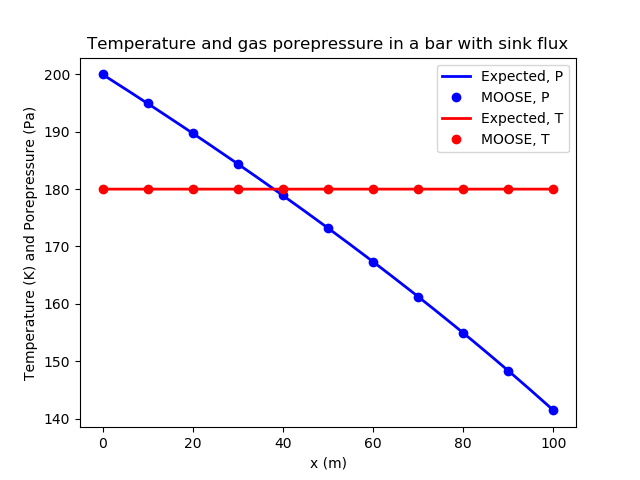
\includegraphics[width=17cm]{nc08.pdf}
\caption{The steady-state porepressure and temperature distributions
  in the bar ($P_{0}=200$ and $T_{0}=180$).  MOOSE agrees well with
  theory illustrating that piecewise-linear fluid and heat
  sinks/sources as well as ideal fluids are correctly implemented in
  MOOSE.}
\label{nc08.fig}
\end{center}
\end{figure}





\end{document}


